\documentclass[11pt,a4paper]{article}
\usepackage{times}
\usepackage[utf8]{inputenc}
\usepackage{url}
\usepackage{ulem}
\usepackage{graphicx}

\begin{document}
\title{RFC : Interfaces for Mechanized Proof Assistants}
\author{Protagonists : Florent {\sc Kirchner},
  Pierre-Yves {\sc Strub}, and Benoît {\sc Boyer}}
\maketitle


\noindent{\large[SCRATCHPAD]}

\section*{IPE - Integrated Proof Environment.}


There should be a {\bf full-screen} mode, and a {\bf presentation} mode
(fullscreen + replayable script + \dots).

We need something similar to {\bf stack and display relevant parts of the
current '.v' file(s), of the library}. [Do we also need to add parts of
the current proof tree?] This "Documentation Panel" could be visible
at all times, or only appear when called (via keyboard shortcut,
icons, etc.). {\it c.f.} Laurent Hubert's implementation of a stacking
Javadoc browser: \url{http://javalib.gforge.inria.fr/test/}. There
should be a way to add various {\bf metadata} to the library (and sync it
into the cloud?).


History of commands should be displayed by {\bf time} of application, and by
{\bf branch}.


Resizing {\bf error pane}, to account for large error messages. \sout{Notice that
the traditional workflow goes like this:}

\begin{itemize}
\item \sout{Look at the goal}
\item \sout{Edit the '.v'}
\item \sout{Optionally, look at the error}
\item \sout{Rince and repeat.} \quad  {\large[INCLUDED BELOW]}
\end{itemize}



We need a heavy subset of the {\bf Emacs command-set}---that is, if such
commands make sense in our interface. And, of course, vi bindings...


Allow users to conduct {\bf in-depth proof development just as well as
in-width} (cf focus, postpone). It should be possible to suspend an
ongoing proof, prove a lemma or a related theorem, and then use it in
the resumed proof. Given the current state of PAs, this means having
multiple instances running side-by-side.


The prover must allow {\bf full script editing} and searching (script =
content of the current '.v'). No "forbidden region".

Make the current {\bf proof zoomable / browsable}. In particular, there
should be a point where we are 'far enough' of the proof to replace it
with an abstract representation. Maybe a stylized tree? Navigation
between goals could use some zazz: the proof display could navigate
between them using a "carousel" effect (think Coverflow). The rotation
axis could be the nearest common ancestor.


Proof development could be highly interactive, with only a {\bf single-line
prompt} to type in proof commands. In this case, the proof script
should be {\bf generated on-demand}. In particular, the IPE could generate
custom/local scripts: for instance, the chain of tactics that lead to
a particular node or leaf of the proof tree (a proof script branch, if
you will).


In the case of a single-line prompt, the IPE should be able to {\bf apply
the input tactics to an arbitrary number} of open goals. This is to
enable simultaneous development of subproofs. The interface should
clearly signal which of these commands succeed, and which fail.


Proof commands are {\bf pre-processed} by the IPE, for purposes such as
providing step-by-step execution (a la Tinycal). As a consequence, the
{\bf proof language used by the IPE} will be a quite {\bf different} beast than
Coq's Ltac (for isntance, the execution of the script "t1;" would be
authorized). In particular, it includes tactics, but could add more
complex features (e.g. a 'next' tactical, and other interface-specific
proof navigation commands).

Interactive proof development is not unlike a debugging
routine. Should we take some cues from Eclipse/Visual Studio?


{\bf Tactic development} requires {\bf a particular edition mode}: tactic
definition differs from proof development. During tactic edition the
documentation must be focused on a specific doc instead of standard
library; however, it might not be necessary to present the user with
the proof tree. The tools provided by Coq for tactics debugging are
poor: limited to step-by-step execution (Ltac Debug On). A good tactic
editor should provide some common features as in standard code
editors. It could be interesting to have a widget to list available
user tactics.

\noindent{\large[/SCRATCHPAD]}

\newpage
\section*{Mockups}
\noindent
Grey areas are uneditable text fields. 


\section*{Coqide}
\noindent 
The current Coqide layout:

\begin{figure}[ht!]
  \centering
  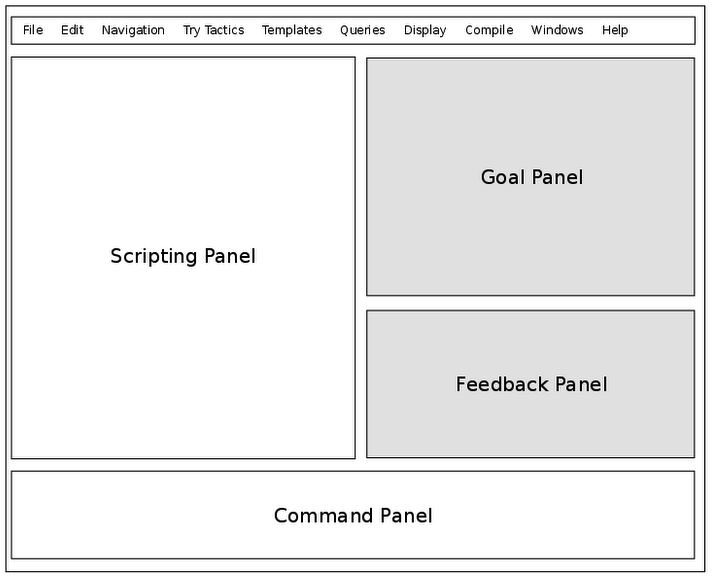
\includegraphics[width=7cm]{files/coqide.png}
  \caption{files/Codeide.svg}
  \label{fig:1}
\end{figure}

In Coqide, you work on your {\bf proof script}. Yet during proof development
you want to work on your {\bf proof tree}.


Remark that the workflow is very circular: one reads the proof state
in the goal panel, then writes a script in the scripting panel, and
take into account potential messages in the feedback panel. Rince and
repeat. This is illustrated by Figure~\ref{fig:2}.

\begin{figure}[ht!]
  \centering
  \includegraphics[width=7cm]{files/Coqide-wflw.png}
  \caption{files/Coqide-wflw.svg}
  \label{fig:2}
\end{figure}

\section*{Prototype - One}
This returns to the concept of toplevel interaction. Note that the
Goal panel in this mockup take the form of a popup overlay; it could
as well be a full-fledged window frame (on the same level as the Doc
Panel and the Proof tree Panel).

\begin{figure}[ht!]
  \centering
  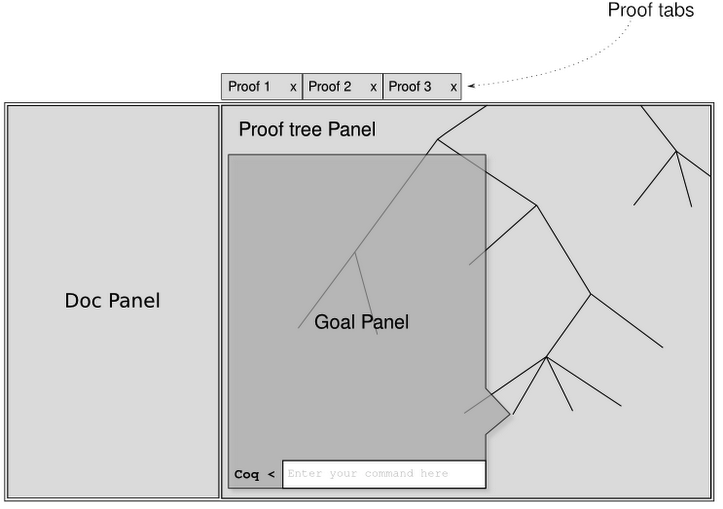
\includegraphics[width=7cm]{files/proto1.png}
  \caption{files/proto1.svg}
  \label{fig:3}
\end{figure}


The diagram (Figure~\ref{fig:4}) shows a use-case where the developer tries to input a proof
command, which fails, displaying a summary error message. The message
can then be viewed in full, if necessary.  

\begin{figure}[ht!]
  \centering
  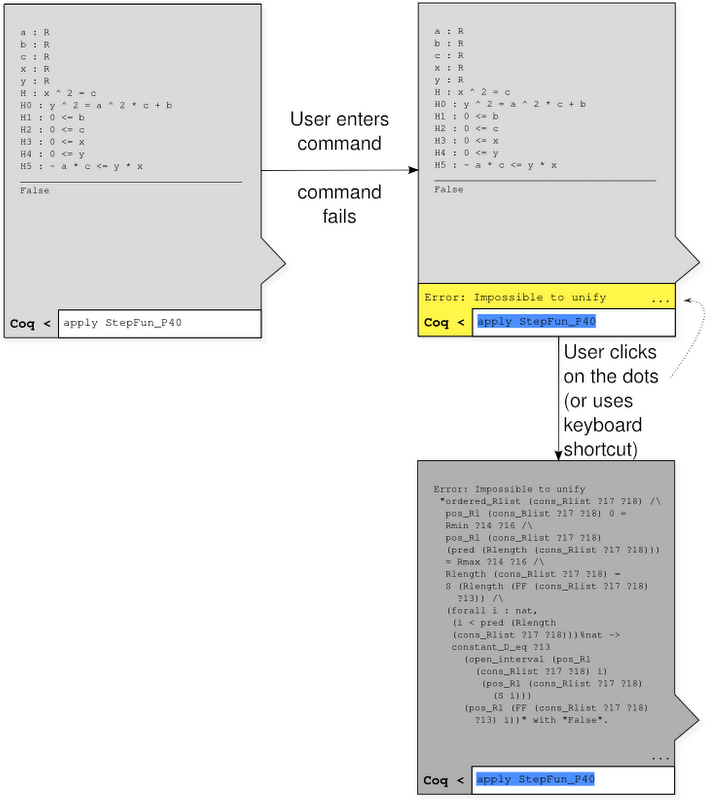
\includegraphics[width=12cm]{files/proto1-goalpanel.png}
  \caption{files/proto1-goalpanel.svg}
  \label{fig:4}
\end{figure}

\newpage

\section*{Docs}
%\url{Florent.kirchner@googlewave.com} and \url{boyer.benoit@googlewave.com}:
\begin{itemize}
\item Une intro à Python pour les programmeurs :\\
  \url{diveintopython.org}

\item Signals+Events sur SO :\\
  \url{stackoverflow.com/questions/2048098/pyqt4-signals-and-slots}

\item Voici le lien qui m'a éclairé sur la programmation des signaux:\\ \url{commandprompt.com/community/pyqt/c1267}\\
  De manière générale, leur GUI Programming with Python\footnote{\url{http://www.commandprompt.com/community/pyqt/book1}} est assez détaillé.
\end{itemize}

\end{document}

%%% Local Variables: 
%%% coding: utf-8
%%% mode: latex
%%% TeX-master: t
%%% TeX-PDF-mode: t
%%% End: 
